\documentclass[11pt]{article}
\usepackage[margin=1in]{geometry}
\usepackage{amsmath,amssymb,booktabs,graphicx,hyperref,xcolor,enumitem}
\usepackage[T1]{fontenc}
\usepackage{lmodern}
\setlist{nosep,leftmargin=*}
\hypersetup{colorlinks=true,linkcolor=black,urlcolor=blue!50!black}
\title{\vspace{-1.5em}Sampled Coverage in RLVR: Findings and a Proposed Warm Start\\[2pt]
\large Research brief, October 30, 2026}
\author{}
\date{}
\begin{document}
\maketitle
\vspace{-3.5em}

\paragraph{Summary.}
We set out to make reinforcement learning with verifiable rewards (RLVR) more diverse, meaning a higher pass@$k$ at a
given pass@1. None of the RL-algorithm changes we tested, and none of the interpretable comparisons with published
checkpoints, met our pre-registered criterion for raising pass@16 at matched pass@1; the outcomes were equivalence of
checkpoint averages, inconclusive comparisons, or comparisons with insufficient reference overlap. A small supervised
fine-tuning (SFT) step before RL, on hard problems with teacher solutions, produced a positive average gap during early
RL: $+1.92$ percentage points (95\% interval [$+0.68$, $+3.12$]). Diagnostics suggest the gain comes with a more even
distribution of success across problems, and a one-seed check found positive offsets at 2,048 tokens. The cause of
the gain and its longer-term persistence are open; we propose a method built on it and the experiments to test it.

\section{Setting and notation}
The core controlled study uses Qwen2.5-Math-1.5B, MATH training problems, 511 MATH test problems, 32 samples per
problem, a 1,024-token answer cap and three RL seeds. Starting models receive 64-sample evaluations, and selected
sensitivity checks use 2,048 tokens. Separate studies evaluate public 1.5B checkpoints at up to 3,072 tokens, 7B
checkpoints at 2,048 tokens, and long-run coverage with 256 samples per problem. RL algorithm: Dr.~GRPO
(group-relative advantages $r-\bar r$, constant normalizer, near on-policy, no KL), 16 problems $\times$ 8 rollouts
per step, 150 steps.
\begin{itemize}
\item \textbf{pass@1} is average single-attempt accuracy; \textbf{pass@16} is the average chance of at least one
correct answer in 16 independent attempts. With $p_x$ the success probability on problem $x$,
pass@$k = \mathbb{E}_x[1-(1-p_x)^k]$, estimated unbiasedly from counts.
\item \textbf{Matched-pass@1 gap}: a checkpoint's pass@$k$ minus the reference's pass@$k$ interpolated at the
checkpoint's pass@1 along the reference trajectory (Dr.~GRPO from the same base and seed), averaged over eligible
checkpoints and seeds. Intervals resample test problems while holding the trained models fixed.
\item \textbf{Decision rules} (fixed in advance): ``curve raised'' requires a pooled estimate of at least $+2$
points, a pooled 95\% interval above zero, positive estimates in all RL seeds and Holm-adjusted $p\le0.05$; where
tested, checkpoint-average equivalence requires the pooled and each seed's 90\% interval inside $\pm2$ points.
Support checks precede interpretation; public-checkpoint departures use a separately registered rule.
\item \textbf{Across-problem spread}: at matched pass@1, pass@$k$ depends on the distribution of success
probabilities across problems; pass@2 $=2\,\mathbb{E}[p]-\mathbb{E}[p^2]$ is a variance diagnostic (at equal mean
accuracy, higher pass@2 means lower variance, i.e.\ success spread more evenly).
\item \textbf{Within-problem answer variety}: distinct normalized incorrect final-answer classes per problem, and the
chance that two parsed incorrect answers to a problem match (averaged over problems with at least two). These do not
describe the variety of reasoning paths or of correct solution methods.
\end{itemize}

\section{Findings so far}
\paragraph{1. Tested RL changes: no registered upward departure.}
We tested positive- and negative-sample reinforcement, sample allocation to uncertain problems, human-solution
prefixes, replay, update-geometry changes, Flat-RLVR (sharpness-aware updates), longer training, and two
outcome-based diversity bonuses (UCB-Con and Batch, Song et al., arXiv 2509.06941). None met the registered
upward-departure criterion; some established equivalence of checkpoint averages, others were inconclusive or lacked
sufficient reference overlap. UCB-Con produced a small increase in distinct incorrect-answer classes ($+0.057$ per
problem); Batch did not demonstrate an increase. Their matched pass@16 gaps were $+0.40$ and $+0.01$ points, and both
met the equivalence rule. In our adaptation, their matched pass@32 gaps ($+0.31$ and $-0.18$) had upper bounds below
the paper's $+1.7$-point reference magnitude; differences in training, model size and implementation limit that
cross-study comparison. For 14 published 7B checkpoints, three primary analyses gave 28 interpreted comparisons
(6 equivalent, 18 inconclusive, 4 downward departures) and 14 with insufficient overlap; none met the upward-departure
criterion.

\paragraph{2. Two kinds of diversity.}
During Dr.~GRPO training (seed 8), the variance of per-problem success rose from 0.033 to 0.130 as pass@1 rose from
21.6\% to 58.1\%, and the chance that two incorrect answers to a problem coincide rose from about 5\% to 14\%. Across
the tested RL conditions, matched pass@2 differences are small (Table~\ref{tab:decomp}), whereas the SFT conditions
show much larger ones; equivalence of both diversity measures to the cross-seed control has not been formally tested.

\begin{table}[h]
\centering\small
\caption{Descriptive checkpoint-average gaps at matched pass@1 (first 32 samples per problem; 90\% bootstrap
intervals for the SFT rows). pass@16 and pass@2 gaps are in percentage points; distinct wrong classes are counts;
collision differences are in probability units. Two of the RL rows (HGm, PG) use two seeds; others use three. SFT
rows cover eligible checkpoints through step 50; R25's registered contrast was not interpreted (support).}
\label{tab:decomp}
\resizebox{\linewidth}{!}{\begin{tabular}{lcccc}
\toprule
Condition & pass@16 (coverage) & pass@2 (spread) & distinct wrong & wrong-answer collision \\
\midrule
Control: Dr.~GRPO seed vs next seed & $+0.14$ & $+0.13$ & $+0.02$ & $+0.000$ \\
10 RL-algorithm conditions (range) & $-0.15$ to $+0.40$ & $+0.08$ to $+0.19$ & $-0.04$ to $+0.09$ & $-0.003$ to $+0.005$ \\
SFT start R25, then RL & $+1.03$ & $+2.62$ [$+2.11$, $+3.16$] & $-0.78$ & $-0.040$ \\
SFT start H25, then RL & $+1.92$ & $+2.39$ [$+1.97$, $+2.82$] & $-1.54$ & $-0.025$ \\
\bottomrule
\end{tabular}}
\end{table}

\paragraph{3. A small SFT start before RL.}
H selects problems with at most four successes in 64 base samples and a surviving teacher solution; R selects the same
number of teacher-covered problems at random, with H's subject mix. Teacher: Qwen2.5-Math-7B-Instruct; solutions have
verifier-correct final answers, but their reasoning is not certified (an audit of 50 found two flawed explanations
and one notation defect). The H pool contains 262 of the 456 low-count problems, including 26 of the 110 with zero
observed successes. At the nominal 25K-token dose, H25 used 48 solutions (27,166 tokens) and R25 used 56 (25,126
tokens). Larger doses (0.5M and 2M tokens) gave pre-RL pass@64 of about 92.6--93.7\% versus 90.0\% for the base, but
their pass@1 (61.6--69.1\%) exceeded the reference's range, so after inspecting those results we amended the design;
the 25K dose was selected by a disclosed validation-only fallback because no screened dose met the primary rule.

H25's mean matched pass@16 gap across eligible checkpoints 1--50 was $+1.92$ points (95\% interval [$+0.68$,
$+3.12$]; Holm $p=0.002$), with positive means in all three RL seeds. The registered ``curve raised'' verdict is
inconclusive because the estimate is below $+2$; the interval still allows effects above that threshold. Post-RL
estimates are descriptively close to the start's own offset ($+1.7$ to $+1.9$), but preservation was not formally
tested. R25's descriptive estimate is $+1.03$; its registered contrast, and therefore the H-versus-R comparison, were
not interpreted because of insufficient support.

\paragraph{4. Budget check: positive offsets remain at 2,048 tokens.}
At 1,024 tokens about 45\% of the starts' answers are cut off. In a one-seed descriptive check, H25's start gap was
$+3.32$ points at 2,048 tokens versus $+1.90$ at 1,024, and its step-50 gap $+2.31$ versus $+1.95$; the step-25
estimate was smaller at the longer budget ($+0.87$ versus $+1.57$), and truncation remained 21--29\%. The positive
offset is not confined to the 1,024-token cap; finishing, formatting and answer extraction remain possible
contributors. Across eligible early-RL checkpoints, the pass@2 gaps were $+2.39$ (H25) and $+2.62$ (R25) against
$+0.13$ in the cross-seed control, suggesting a more even success profile; the conditional wrong-answer collision was
lower by 2.5 and 4.0 percentage points. Distinct-class counts fell, but they depend on how incorrect samples are
distributed across problems; these measurements do not establish the cause of the coverage gain.

\paragraph{5. What did not hold.}
A frozen per-problem model fitted on RL from the base overestimated H25's gap ($+6.69$ forecast versus $+1.92$
observed; registered verdict ``forecast fails''), so it is not a validated predictor for new starts. At the same
nominal dose, an on-policy-distillation start (Dong et al., arXiv 2609.28145) showed no clear positive starting offset
($+0.34$, 90\% interval [$-0.73$, $+1.34$], against reference seed 8); its post-RL results are being finalized.

\begin{figure}[h]
\centering
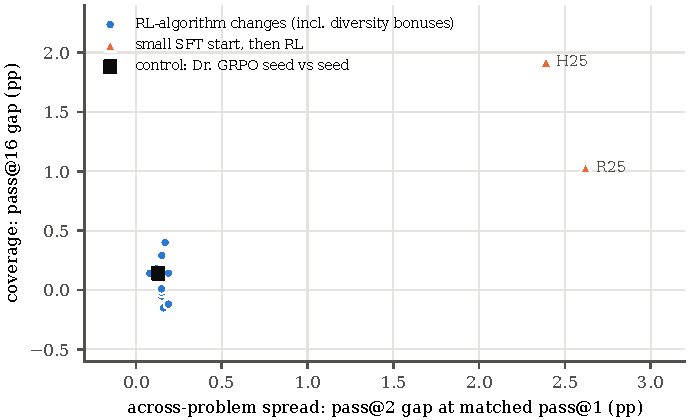
\includegraphics[width=0.66\linewidth]{decomposition.pdf}
\caption{Descriptive mean gaps in pass@16 and pass@2 at matched pass@1. The SFT conditions show larger gaps than the
tested RL conditions; this association does not establish a causal mechanism.}
\label{fig:decomp}
\end{figure}

\section{Why this pattern might occur}
At equal average accuracy, moving a small amount of success probability from easier toward harder problems can raise
repeated-sampling coverage: for small changes $\delta_x$ with $\mathbb{E}[\delta_x]=0$, the first-order pass@$k$
gap is $\mathrm{Cov}_x\big(k(1-p_x)^{k-1},\delta_x\big)$. This describes a local change in success probabilities; it
does not prove that different RL methods follow the same trajectory. Standard Dr.~GRPO gets no direct reward
advantage from a group whose rewards are all equal, so rarely solved problems give it little learning signal
(if each of $M$ draws succeeds with probability at most $\epsilon$, the chance of any success is at most
$\min(1, M\epsilon)$); training on other problems and added bonuses can still improve hard problems. Rollout variety
is what RLVR learns from, and RL reduces it by sharpening. The experiments suggest that changing the starting
success profile is useful, while leaving room for effective RL-time interventions not yet tested.

\section{Proposed direction: a coverage-targeted warm start}
\paragraph{Method.} Before RL, run a small SFT step (about 25K response tokens) drawing problems with replacement from
the 3,550 problems with archived teacher solutions, with weights $16(1-\hat p_x)^{15}$, a local measure of pass@16
sensitivity to success probability; $\hat p_x$ comes from 64 base samples per training problem (Beta-prior
shrinkage). Within this pool, the weights put about 9.1\% of draws on problems with zero observed successes, 44.0\% on
counts 1--4, 45.3\% on counts 5--16 and 1.6\% on higher counts (uniform: 0.7\%, 6.6\%, 36.6\%, 56.0\%). Then run
standard RL unchanged. If self-SFT succeeds, it motivates a teacher-free variant on problems with verified base
solutions; extending it to zero-count problems would need further sampling or another solution source.

\paragraph{Experiments, in order.}
\begin{enumerate}
\item \textbf{Controls at the same 25K dose} (one RL seed through step 50 each; estimated 3 hours, about \$95).
Self-SFT and teacher SFT use the same restricted prompts with approximately matched lengths. Format-only SFT
supervises boxing delimiters and the stop token, masking reasoning and answer content; its null result is informative
only if boxing increases and truncation falls. A corrupted-answer control changes the final boxed label while
retaining reasoning and earlier answers. A second SFT seed tests reproducibility. A control receives additional RL
seeds if its supported seed-8 gap is at least $+0.96$ points or if it enters a confirmatory contrast (self-SFT and
teacher SFT get three seeds together).
\item \textbf{Head-to-head.} Coverage-weighted SFT against uniform sampling from the same eligible pool under the
same settings, hard-only selection and TailSFT (arXiv 2608.25756), with matched nominal response-token budgets
(actual tokens, updates and preparation costs reported) and plain Dr.~GRPO as the reference without SFT; independent
SFT starts and three RL seeds; pass@16 at matched pass@1 (primary), pass@2 (diagnostic), deeper sampling on hard
problems; 1,024 and 2,048 tokens.
\item \textbf{Timing ablation.} The same solutions and SFT updates interleaved during RL (one SFT batch every five
RL steps) instead of before it. If preparation before RL outperforms interleaving, that favors the pre-RL schedule
over the tested interleaving schedule.
\item \textbf{Persistence and replication.} Longer Dr.~GRPO references (700 steps) aim to extend the accuracy range;
later checkpoints are interpreted only where overlap is sufficient and reproducibility checks pass. A second model
family tests replication.
\end{enumerate}

\paragraph{Decision point and risks.} After about four weeks: if the coverage-weighted start reproducibly beats
uniform SFT and TailSFT, the paper is a method paper; otherwise it is a measurement paper on coverage at matched
accuracy. If random and targeted SFT perform similarly and both show positive gaps, the contribution concerns
preparation before RL in the tested setting, without a demonstrated targeting benefit. Formatting may explain part or
all of the gain. Durations and costs are planning estimates; the submission target is ICML 2027 (late January).

\section{Limits of the current evidence}
These evaluations use Qwen2.5-Math-based models on MATH. Some public 1.5B checkpoints were evaluated at 3,072 tokens;
locally run RL experiments extend to 1,000 steps. Later core 1.5B pass@16 values are roughly 86--89\%, leaving little
headroom. The primary 32-sample comparison does not measure pass@256; in a separate 256-sample study, a 1,000-step
run's gain over the base was $+1.96$ points (unadjusted 95\% interval [$+0.39$, $+3.72$]) but missed the registered
multiplicity-adjusted criterion, a comparison not matched in pass@1. Several comparisons are inconclusive or lack
reference overlap rather than being equivalent. The SFT-start effect rests on one start per selection and three RL
seeds; its persistence beyond step 50 and its source are being tested.

\end{document}
